\section*{A First Look}
\begin{figure}[htp]
\centering
\begin{subfigure}{0.3\textwidth}
    \centering
    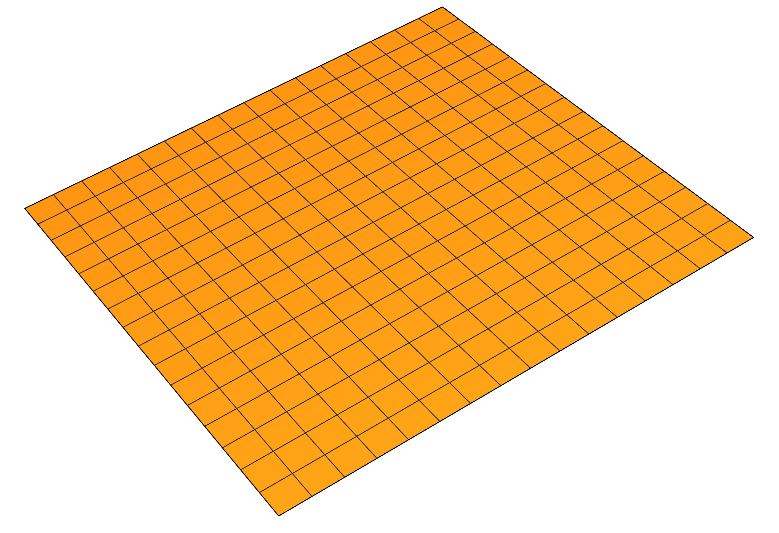
\includegraphics[width=\textwidth]{picture/week4/plane.pdf}
    \caption{Plane}
\end{subfigure}
\begin{subfigure}{0.2\textwidth}
    \centering
    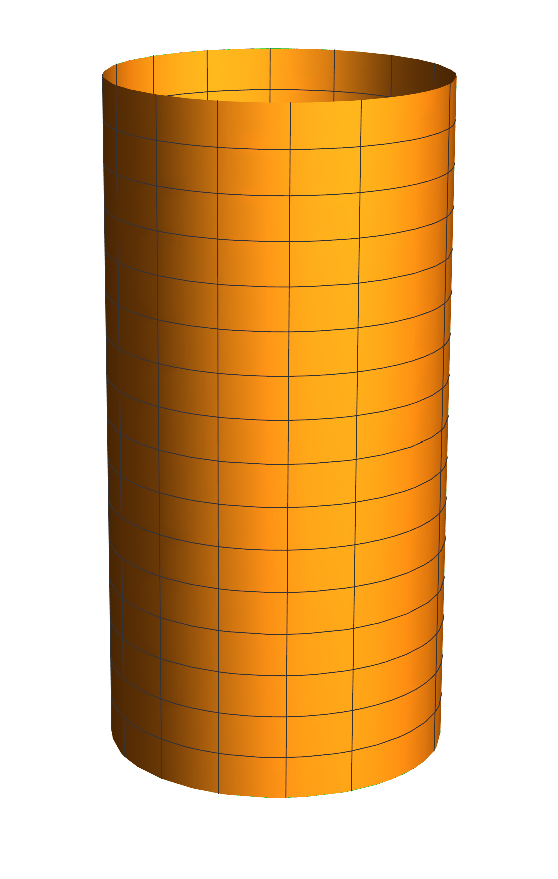
\includegraphics[width=\textwidth]{picture/week4/cylinder.pdf}
    \caption{Cylinder}
\end{subfigure}
\begin{subfigure}{0.4\textwidth}
    \centering
    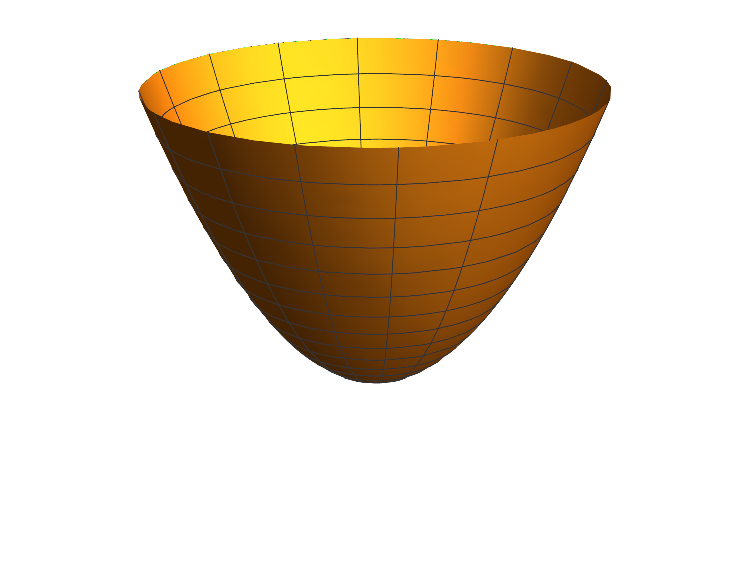
\includegraphics[width=\textwidth]{picture/week4/paraboloid.pdf}
    \caption{Paraboloid}
\end{subfigure}
\begin{subfigure}{0.3\textwidth}
    \centering
    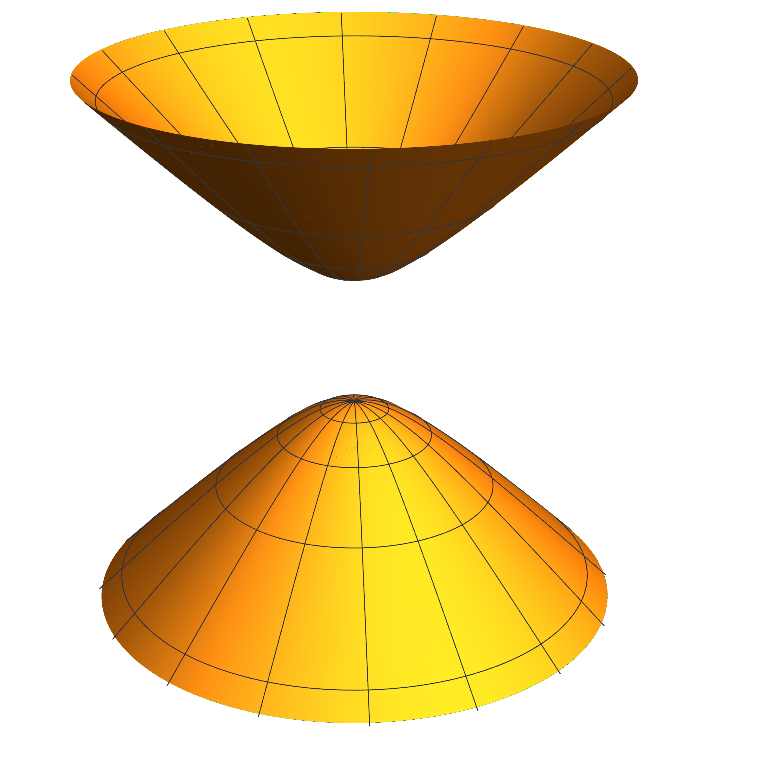
\includegraphics[width=\textwidth]{picture/week4/hyperboloid.pdf}
    \caption{Hyperboloid}
\end{subfigure}
\begin{subfigure}{0.2\textwidth}
    \centering
    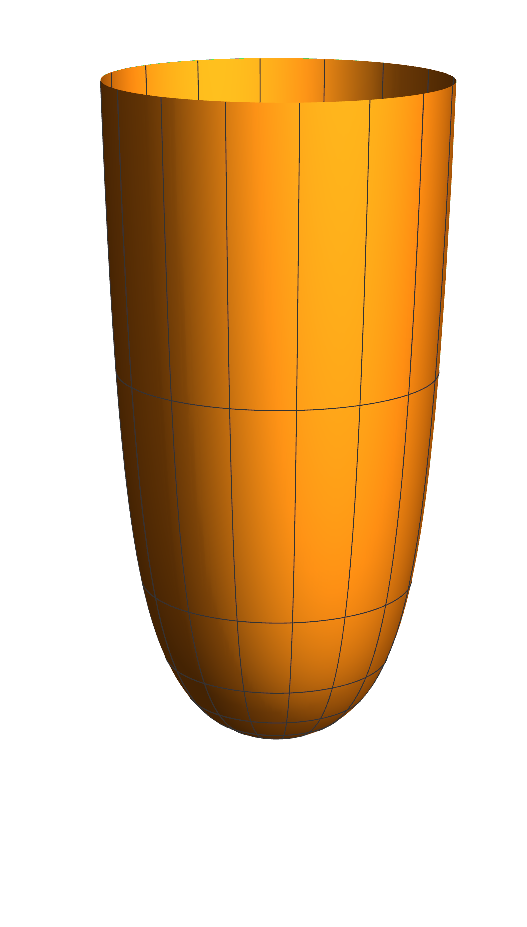
\includegraphics[width=\textwidth]{picture/week4/cigar.pdf}
    \caption{Cigar soliton}
\end{subfigure}
\caption*{Surface collection 1}
\end{figure}

\begin{figure}
\centering
\begin{subfigure}{0.25\textwidth}
    \centering
    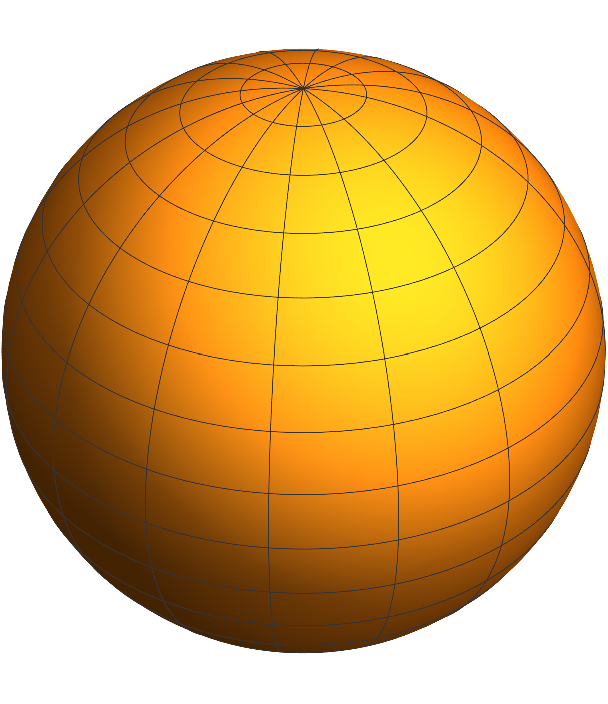
\includegraphics[width=\textwidth]{picture/week4/sphere.pdf}
    \caption{\(\mathbb{S}^2\)}
\end{subfigure}
\begin{subfigure}{0.35\textwidth}
    \centering
    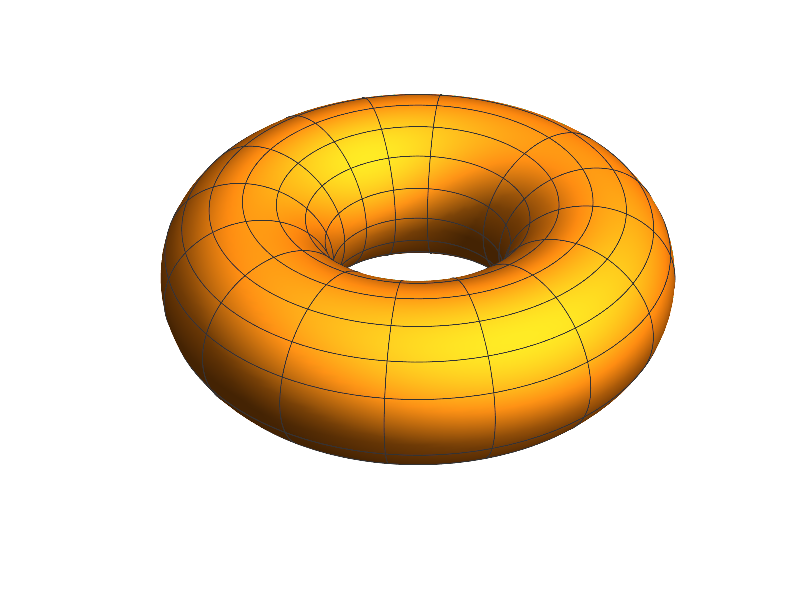
\includegraphics[width=\textwidth]{picture/week4/torus.pdf}
    \caption{\(\mathbb{T}^2\)}
\end{subfigure}
\begin{subfigure}{0.35\textwidth}
    \centering
    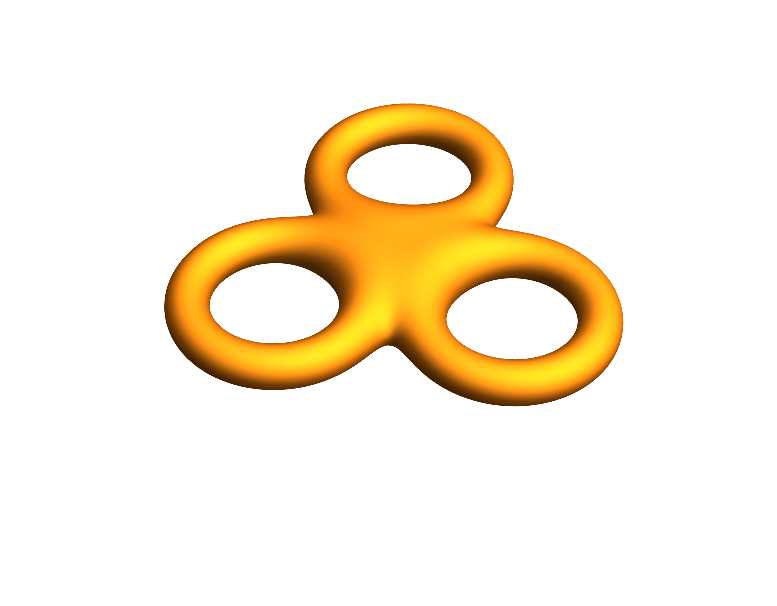
\includegraphics[width=\textwidth]{picture/week4/torus3.pdf}
    \caption{\(\Sigma_g\) for \(g=3\)}
\end{subfigure}
\caption*{Surface collection 2}
\end{figure}

\begin{figure}
\centering
\begin{subfigure}{0.45\textwidth}
    \centering
    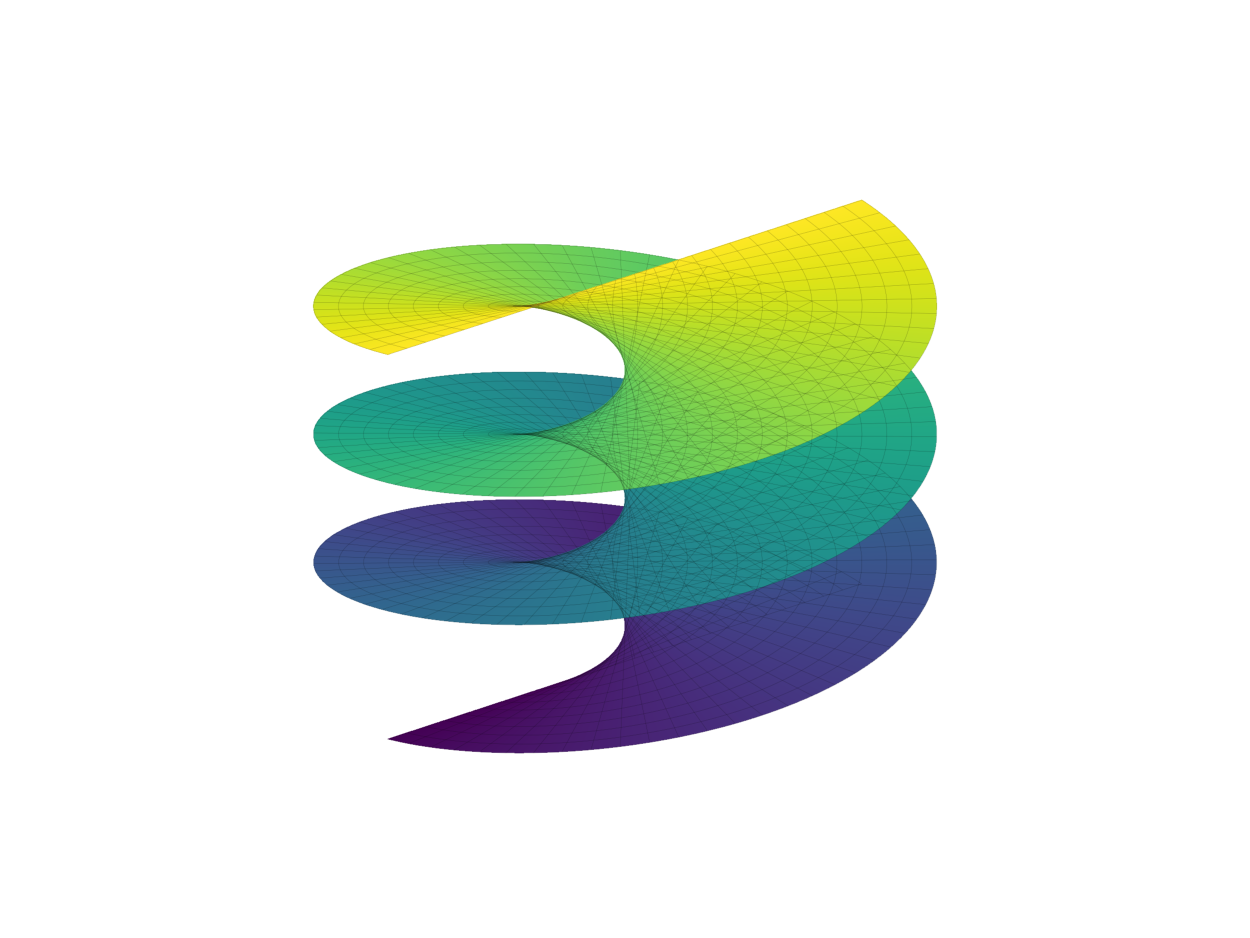
\includegraphics[width=\textwidth]{picture/week4/helicoid.pdf}
    \caption{Helicoid}
\end{subfigure}
\begin{subfigure}{0.45\textwidth}
    \centering
    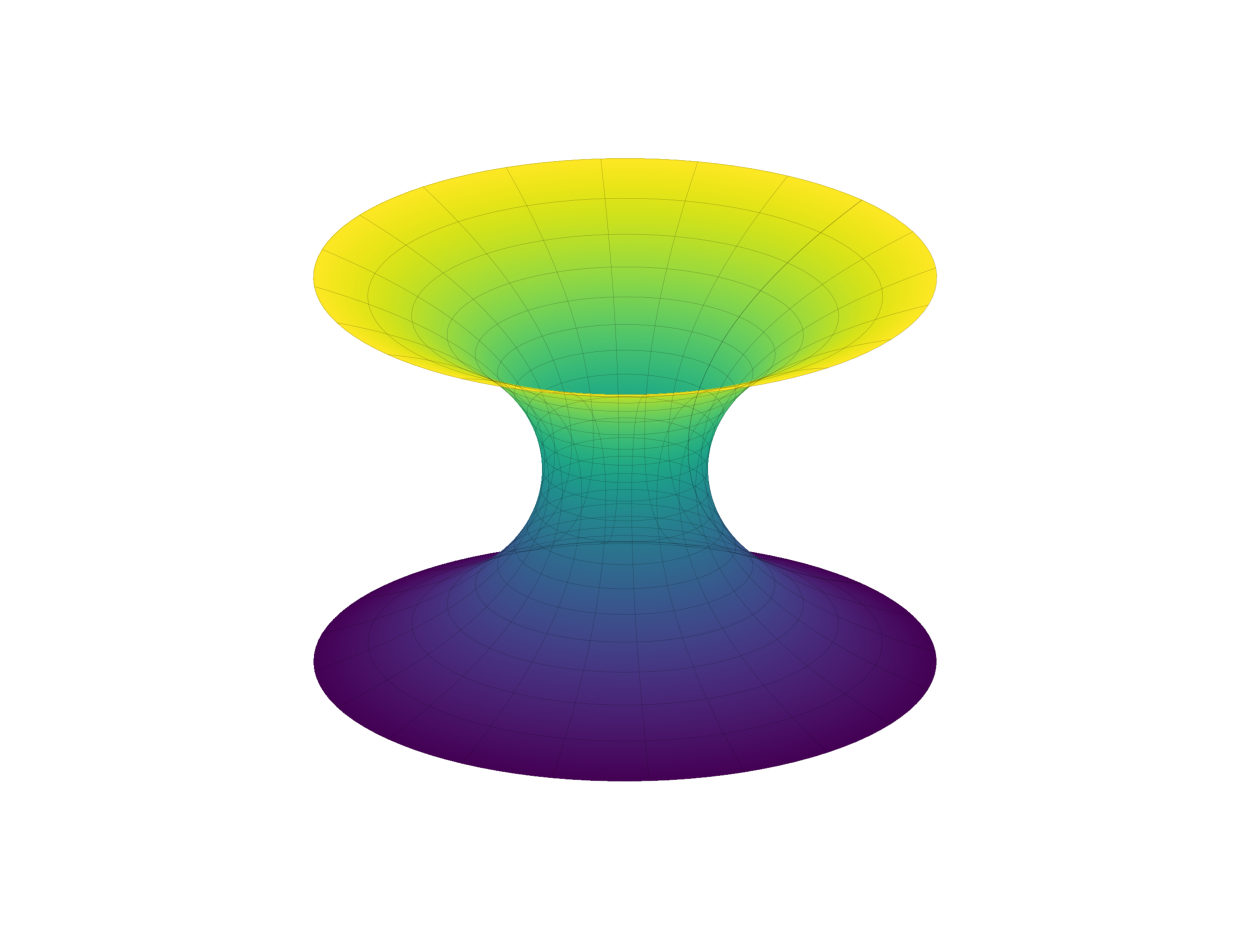
\includegraphics[width=\textwidth]{picture/week4/catenoid.pdf}
    \caption{Catenoid}
\end{subfigure}
\begin{subfigure}{0.5\textwidth}
    \centering
    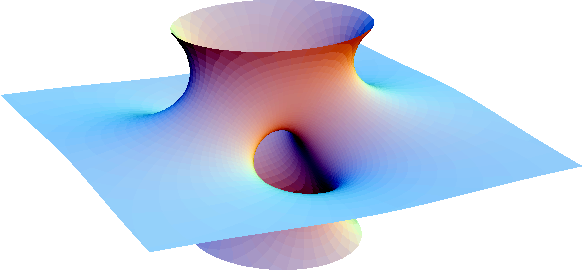
\includegraphics[width=\textwidth]{picture/week4/costa.pdf}
    \caption{Costa minimal surface}
\end{subfigure}
\begin{subfigure}{0.4\textwidth}
    \centering
    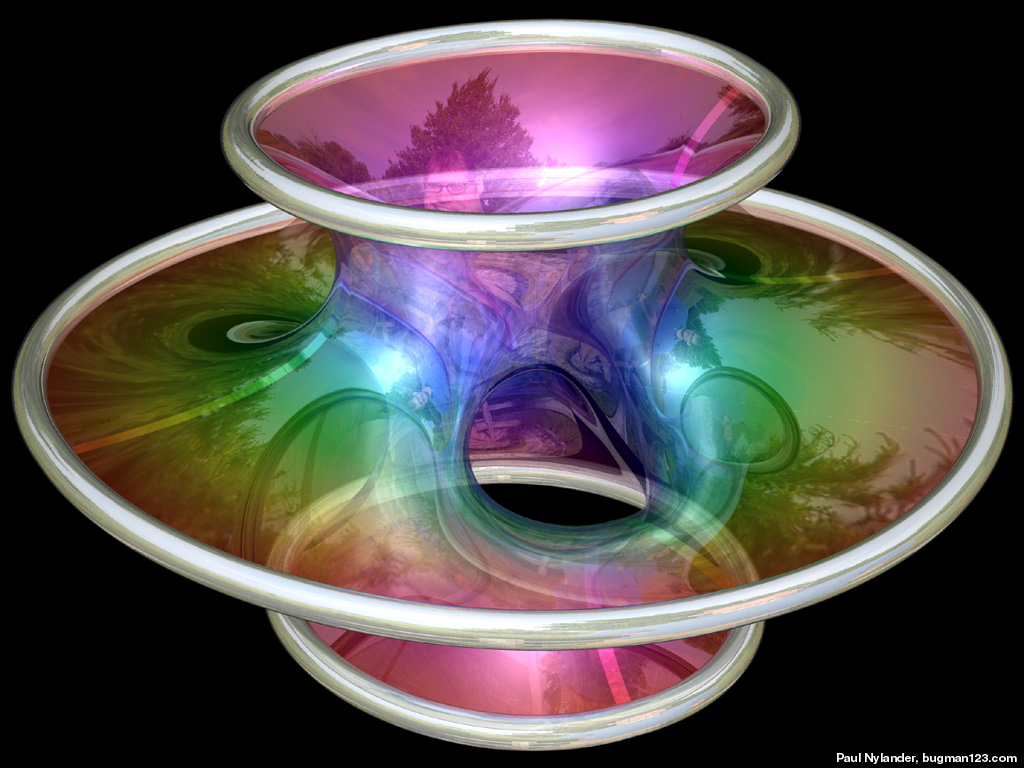
\includegraphics[width=\textwidth]{picture/week4/Costa-large.jpg}
    \caption{Soap bubble}
\end{subfigure}
\caption*{Surface collection 3}
\end{figure}

\begin{figure}
\centering
\begin{subfigure}{0.3\textwidth}
    \centering
    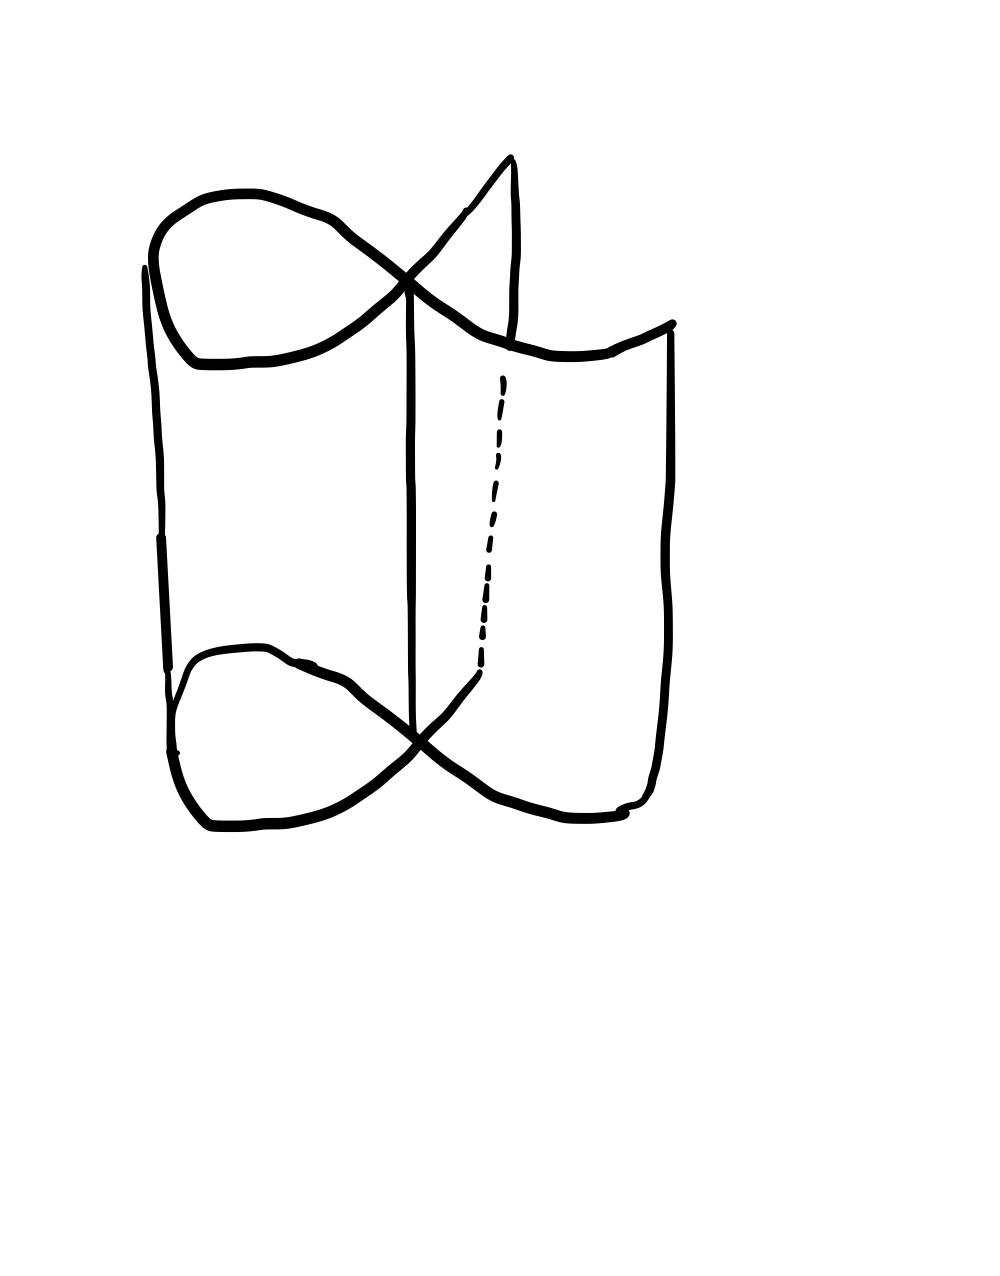
\includegraphics[width=\textwidth]{picture/week4/self-intersetcion.png}
    \caption{Self-intersected}
\end{subfigure}
\begin{subfigure}{0.35\textwidth}
    \centering
    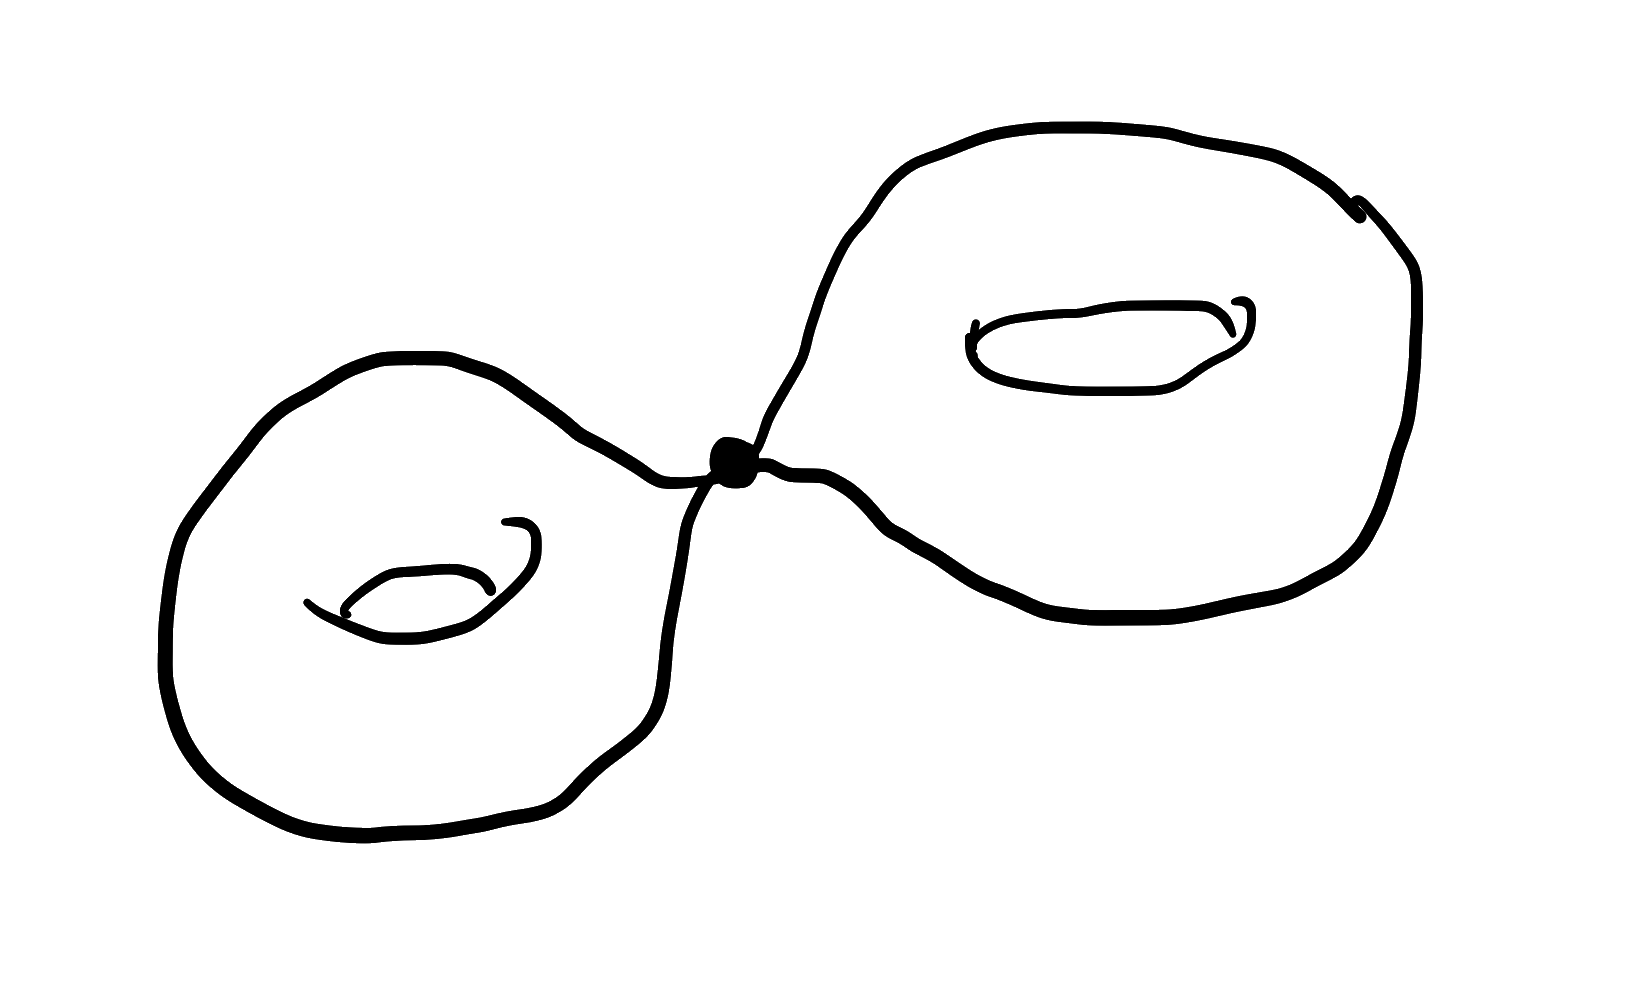
\includegraphics[width=\textwidth]{picture/week4/node.png}
    \caption{Nodal surfaces}
\end{subfigure}
\begin{subfigure}{0.3\textwidth}
    \centering
    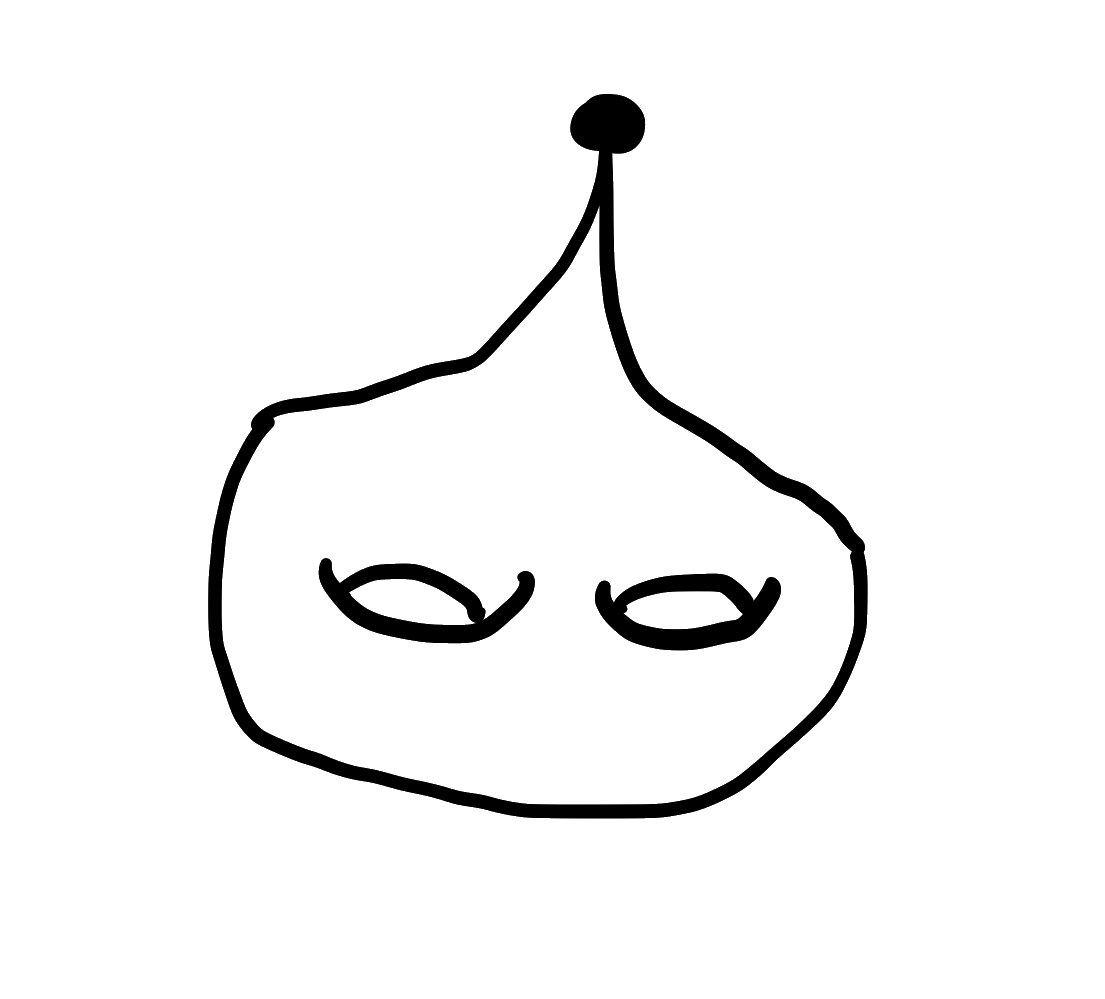
\includegraphics[width=\textwidth]{picture/week4/cusp.png}
    \caption{Cusp}
\end{subfigure}
\caption*{``Surface'' collection 4}
\end{figure}

\begin{example}\hfill
\begin{itemize}
    \item Collection 1 are complete non-compact surfaces.
    \item Collection 2 are compact surfaces without boundary (closed).
    \item Collection 3 are so called minimal surfaces, a very important class
        of surfaces. The term ``minimal'' intuits smallest area in certain sense.
    \item There are surfaces will NOT be investigated in this course, the ones with
        self-intersection, node points or cusps, and non-orientable surfaces.
\end{itemize}    
\end{example}

\section{Definition of Regular Surface}

\begin{definition}[Regular surfaces in \(\mathbb{R}^3\)]\hfill\par
    A subset \(S\subset \mathbb{R}^3\) is called a regular surface, if \(\forall\,p
    \in S\), \(\exists\, V\subset\mathbb{R}^3\) neighborhood of \(p\), an open set
    \(U\subset \mathbb{R}^2\) and a trivialization map \[
        F\colon U\to V\cap S
    .\] \st\ \(F\) is smooth, homeomorphism onto its image, and regular.
\end{definition}
\begin{remark}\hfill
\begin{enumerate}[(1)]
    \item \(F\) is homeomorphism means both \(F\) and \(F^{-1}\) are continuous map.
    \item \(F\) is ``regular'' means \(\forall\,p\in U\), \(\dif F_p\) is an 
        injection as linear map \(\mathbb{R}^2\to \mathbb{R}^3\).
\end{enumerate}
\end{remark}

Let's see what the term ``regular'' means:

Assume \(F\) is written as \(F(u,v)=(x(u,v),y(u,v),z(u,v))\), at \(p\in U\), \[
    \dd{F_p}\colon T_p U\to T_{F(p)}S
\] is a linear map. On \(\mathbb{R}^2\), coordinate vector fields \(\{\pdv{u},
\pdv{v}\}\) form a basis. On \(\mathbb{R}^3\) we also have standard basis
\(\{\pdv{x},\pdv{y},\pdv{z}\}\). Then \[
    \dd{F_p}\begin{bmatrix}
        \pdv{u}\\ \pdv{v}
    \end{bmatrix}
    =\begin{bmatrix}
        \pdv{x}{u} & \pdv{y}{u} & \pdv{z}{u} \\ 
        \pdv{x}{v} & \pdv{y}{v} & \pdv{z}{v}
    \end{bmatrix}
    \begin{bmatrix}
        \pdv{x}\\ \pdv{y}\\ \pdv{z}
    \end{bmatrix}
.\] Hence
\begin{align*}
    \dd{F_p}\text{ is injective}
    \iff & \ker\dd{F_p}=0 \\
    \iff & \pdv{(x,y,z)}{(u,v)}\text{ has rank 2} \\
    \iff & \pdv{F}{u}\text{ \& }\pdv{F}{v}\text{ are linearly independent} \\
    \iff & \pdv{F}{u}\times \pdv{F}{v}\neq 0. \\
    & \text{\small\itshape\/ (Geometrically this defines the normal vector field} \\
    & \text{\small\itshape\/ of the tangent plane)} \\
    \iff & \text{ One of the following minors is non-zero:}\\
    & \quad\left|\pdv{(x,y)}{(u,v)}\right|,\quad\left|\pdv{(x,z)}{(u,v)}\right|,
    \quad\left|\pdv{(y,z)}{(u,v)}\right|
\end{align*}
{\small\itshape
    (Geometrically, this means \((u,v)\) can be viewed as coordinate at \(p\in S\)
    via \(F\). In fact, since ``\(\dd{F_p}\) is injective'' is an open condition,
    \((u,v)\) serves as a local coordinate chart in a neighborhood of \(p\))
}

We also call \(F\) to be a local parametrization of \(S\). Note that such \(F\)
is usually not globally defined.

From the definition, we see a regular surface in \(\mathbb{R}^3\) is characterized
by at each point, we can find a ``smooth'' slice chart in a neighbourhood of the
point. The term ``slice chart'' means coordinate chart with local part of the
surface containing in the chart as a slice.

\begin{question}
    Consider two points \(p,q\) on the surface, live close to each other. It might
    happen that their corresponding coordinate chart overlap. Then in the
    intersection of two charts, there are two different parametrizations. What
    relation between these two parametrizations should be?
\end{question}
% Figure here

Set-up: \(F_1\colon U_1\to V_1\cap S,\ (u,v)\mapsto F_1(u,v)\),\hfill \(F_2\colon
U_2\to V_2\cap S,\ (\alpha,\beta)\mapsto F_2(\alpha,\beta)\)

Let \(W=V_1\cap V_2\cap S\), since \(F_i\) is homeomorphism, \(F_1^{-1}(W)\subset U,
\ F_2^{-1}(W)\subset U_2\).

\noindent\underline{\textbf{Claim:}} (Very important).\par
\(G=F_2^{-1}\circ F_1\colon F_1^{-1}(W)\to F_2^{-1}(W)\) is a diffeomorphism,\ie\ 
both \(G\) and \(G^{-1}\) are smooth functions.

The importance of this claim leads us to give an intrinsic definition of a regular
surface \(S\). \ie\ a regular surface is obtained by padding up open sets in
\(\mathbb{R}^2\), in a smooth way. Later in differential geometry course, we'll
define a smooth manifold by such intrinsic definition. The diffeomorphism \(G\)
above is called the transition map. Different property of \(G\) determines different
structure. If \(G\) is only a homeomorphism, then \(S\) is a topological surface.
If \(G\) is a bi-holomorphism, then \(S\) is a complex surface.

The proof of the claim needs the inverse function theorem.
\begin{theorem}[Inverse function thm]
    \(U\subset \mathbb{R}^n\) open. \(F\colon U\to \mathbb{R}^n\) is a \(C^1\) map,
    \(p\in U\). If \(\dd{F_p}\colon \mathbb{R}^n\to \mathbb{R}^n\) is an isomorphism,
    then there is a neighbourhood of \(p\) and a neighbourhood of \(F(p)\).
    \st\ \(F\colon V\to W\) is invertible. Moreover \(F^{-1}\) is also \(C^1\). If
    condition is substituted to \(F\) smooth, then \(F^{-1}\) has same smoothness.
\end{theorem}

\begin{remark}
    From linear algebra, a linear operator on finite dimensional vector space
    is injective iff it's surjective. Hence, it's sufficient to check \(\det(\dd{F_p})
    \neq 0\), \ie\ \(\dd{F_p}\) is non-singular.
\end{remark}

\textbf{\color{red}!!} A priori, we don't know if \(F_2^{-1}\) is smooth, since we
have not defined what ``smooth map'' on a surface mean.

\begin{proof}[Proof of claim]
    Since \(F_1\) and \(F_2\) are homeomorphism, \(G,G^{-1}\) are continuous.
    \(S\) is a regular surface, so at \(p\in U_1\), \((\dd{F_1})_p\colon\mathbb{R}^2
    \to \mathbb{R}^3\) is injective. W.L.O.G. we can assume \[
        \left|\pdv{(x,y)}{(u,v)}\right|\neq 0\text{ at }p
    .\] Consider a map \(h\colon F_1^{-1}(W)\times (-\eps,\eps)\to \mathbb{R}^3,
    (u,v,t)\mapsto (x(u,v),y(u,v),z(u,v)+t)\). Then \(h\) has Jacobian \[
        \det \begin{bmatrix}
            x_u & y_u & z_u \\
            x_v & y_v & z_v \\
            0 & 0 & 1
        \end{bmatrix}
        =\det\begin{bmatrix}
            x_u & y_u \\
            x_v & y_v 
        \end{bmatrix}\neq 0 \text{ at }p
    .\] By inverse function theorem, \(\exists\) a neighbourhood \(D\subset
    \mathbb{R}^3\) of \((p,t)\) \st\ \(h\) is invertible on \(D\), and \(h^{-1}\)
    smooth. Now since \(F_1^{-1}\circ F_2=\eval{h^{-1}\circ F_2}_{t=0}\), and RHS
    is smooth, we conclude that \(F_1^{-1}\circ F_2\) is smooth. Similarly, \(G^{-1}\)
    is smooth.
\end{proof}

Now we give an intrinsic definition (No need to assume \(S\subset \mathbb{R}^3\)).
\begin{definition}
    Topological space \(S\) (second countable, Hausdorff) is called a regular surface
    if \(S\) has a covering \(\{V_\alpha,f_\alpha\}\) \st\ 
    \begin{enumerate}[(1)]
        \item \(f_\alpha\colon V_\alpha\to f_\alpha(V_\alpha)\overset{\text{open}}
            \subset \mathbb{R}^2\) is a homeomorphism.
        \item If \(V_\alpha\cap V_\beta\neq \emptyset\), then \[
            f_\beta\circ f_\alpha^{-1}\colon f_\alpha(v_\alpha\cap V_\beta)\to 
            f_\beta(V_\alpha\cap V_\beta)
        \] is a diffeomorphism, called the transition map.
    \end{enumerate}
\end{definition}
\begin{remark}
    In higher dimension, this definition yields ``smooth manifold''.
\end{remark}

\section{Examples of Regular Surfaces}

\begin{example}[1]
    \(\mathbb{R}^2\hookrightarrow\mathbb{R}^3\) is a regular surface with (trivial)
    global parametrization \[
        F(x,y)=(x,y,0)
    .\] 
\end{example}

\begin{example}[2]
    \label{charts on unit sphere}
    Standard 2-sphere \(\mathbb{S}^2=\{(x,y,z):x^2+y^2+z^2=1\}\). This is a very
    important example, we'll give (local) parametrization for \(\mathbb{S}^2\)
    in 3 ways.
\end{example}
\noindent (a) Parametrization induced from \(\mathbb{R}^3\).

If the point is on upper hemisphere, let \(U=\{x^2+y^2<1\}\), \[
    F_1\colon U\to \mathbb{S}^2,\ (x,y)\mapsto (x,y,\sqrt{1-x^2-y^2}).
\] Check definition:

\(F_1\) is smooth \checkmark{}. 

\(F_1\colon U\to F_1(U)\) is homeomorphism, since \(F_1^{-1}\) is
projection onto \(xy\)-plane, is also continuous.

\(F_1\) is regular: \[
    \pdv{F_1}{x}=(1,0,-\frac{x}{\sqrt{1-x^2-y^2}}),\quad
    \pdv{F_1}{y}=(0,1,-\frac{y}{\sqrt{1-x^2-y^2}})
.\] Clearly they are linearly independent.

Similarly, if the point is on lower hemisphere, we have \[
    F_2\colon U\to \mathbb{S}^2,\ (x,y)\mapsto (y,x,-\sqrt{1-x^2-y^2})
.\] However, \(F_1(U)\cup F_2(U)\) can not fully cover \(\mathbb{S}^2\), points on
the equator are left. To cover them, we add 4 more charts:
\begin{align*}
    F_3(y,z)&= (\sqrt{1-y^2-z^2},y,z) &&\text{(front hemisphere)} \\
    F_4(y,z)&= (-\sqrt{1-y^2-z^2},z,y) &&\text{(back)} \\
    F_5(z,x)&= (x,\sqrt{1-x^2-z^2},z) &&\text{(right)} \\
    F_6(z,x)&= (z,-\sqrt{1-x^2-z^2},x) &&\text{(left)}
\end{align*}
We can check \(F_2\)-\(F_6\) also satisfy the definition. Hence, we have given each
point a smooth chart, and \(\mathbb{S}^2\) is regular.
\begin{exercise}
    Check transition maps between \(F_1\)-\(F_6\) are smooth.
\end{exercise}

\noindent (b) Geographical parametrization.

% Maybe picture here
Let \(U=\{(\theta,\vphi)\in \mathbb{R}^2:0<\theta<2\pi,0<\vphi<\pi\}\), 
\begin{align*}
    &F_1\colon U\to \mathbb{S}^2,\ (\theta,\vphi)\mapsto 
    (\cos\theta\sin\vphi,\sin\theta\sin\vphi,\cos\vphi)
    \quad\text{(missing half of }\{y=0\}\cap \mathbb{S}^2\text{)}\\ 
    &F_2\colon U\to \mathbb{S}^2,\ (\theta,\vphi)\mapsto 
    (\sin\theta\sin\vphi,\cos\vphi,\cos\theta\sin\vphi)
    \quad\text{(missing half of }\{x=0\}\cap \mathbb{S}^2\text{)}\\ 
    &F_3\colon U\to \mathbb{S}^2,\ (\theta,\vphi)\mapsto 
    (\cos\vphi,\cos\theta\sin\vphi,\sin\theta\sin\vphi)
    \quad\text{(missing half of }\{z=0\}\cap \mathbb{S}^2\text{)}
.\end{align*}
Clearly \(\mathbb{S}^2\subset F_1(U)\cup F_2(U)\cup F_3(U)\), each \(F_i\) is smooth
and regular. To see they are homeomorphism, we can compute e.g. \[
    F_1^{-1}(x,y,z)=(\arccos \frac{x}{\sqrt{x^2+y^2}}, \arccos z)
.\] 

\noindent (c) Stereographic parametrization.

Consider the ray connecting North Pole \((0,0,1)\) and point \((x,y,z)\) on
\(\mathbb{S}^2\). Then there is a unique point \((u,v)\) on \(xy\)-plane on the
ray, the projection is given by \[
    p_N\colon \mathbb{S}^2\setminus\{N\}\to \mathbb{R}^2,
    \quad (x,y,z)\mapsto (\frac{x}{1-z},\frac{y}{1-z})=\colon(u,v)
\] which is rational map, with inverse \[
    p_N^{-1}(u,v)=(\frac{2u}{1+u^2+v^2},\frac{2v}{1+u^2+v^2},1-\frac{2}{1+u^2+v^2})
\] also rational and normal.

Similarly consider the projection from \(S=(0,0,-1)\), \(p_S(x,y,z)=(\frac{y}{1+z},
\frac{x}{1+z})\), these two charts can cover \(\mathbb{S}^2\).

\begin{exercise}
    Check the transition function \[
        p_S\circ p_N^{-1}=(\frac{u}{u^2+v^2},\frac{v}{u^2+v^2})
    .\] 
\end{exercise}

\begin{remark}
    In the stereographic projection parametrization, if we identify \(\mathbb{R}^2\)
    with \(\mathbb{C}^1\), and introduce complex coordinate \[
        w_1=\frac{x}{1-z}+\frac{y}{1-z}i,\quad
        w_2=\frac{x}{1+z}-\frac{y}{1+z}i
    .\] Then we can check \[
        w_1\cdot w_2=1\quad \text{and} \quad
        p_S\circ p_N^{-1}(w_1)=w_2
    .\] In this way, we have given a ``complex structure'' on \(\mathbb{S}^2\),
    the resulting surface is an 1 dim complex manifold, called \(\mathbb{CP}^1\).
    You'll learn more abort \(\mathbb{CP}^n\) in complex / algebraic geometry.
\end{remark}

\textbf{\color{red}!!} \(\mathbb{S}^2\) is a very important example in geometry. One
should keep this example in mind and try to understand and explore it in studding
geometry. \(\mathbb{S}^2\) is a (strictly) convex surface, has maximal number
of \(\mathbb{S}^1\) action (This tells the moment polytope is a line segment).
It has 3-rotation axis (3 Killing vector fields). It looks the same everywhere
(homogeneous). However, since every circle on \(\mathbb{S}^2\) can shrink to a point,
without obstruction, \ie\ \(\pi_1(\mathbb{S}^2)=0\), the fundamental group does not
play a role here.

\begin{example}[3]
    Graph of a function, \ie\ \((x,y,z=f(x,y))\) is a regular surface. More
    generally, if a surface \(S\) can be expressed (locally or globally) as graph
    of smooth functions, then \(S\) is a regular surface.
\end{example}
Parametrization is given by \[
    F\colon U\to S,\quad (x,y)\to (x,y,f(x,y))
.\] We have 
\begin{enumerate}[(a)]
    \item \(F\) is smooth \checkmark{}
    \item \(F\) is homeomorphism, \(F^{-1}(x,y,z)=(x,y)\).
    \item \(F\) is regular \(\det\mathrm{Jac}(\dd{F})=1\).
\end{enumerate}

\begin{example}[4]
    More generally, the level set of a smooth function \(f(x,y,z)\) at a
    \underline{regular} \underline{value} is a regular surface.
\end{example}

\begin{definition}[Critical point (value) \& regular point (value)]
    Let \(F\colon U\subset \mathbb{R}^m\to \mathbb{R}^n\) be smooth map.
    \begin{itemize}
    \item If \(\dd{F_p}\colon\mathbb{R}^m\to \mathbb{R}^n\) is surjective, \ie 
        \(\rank\dd{F_p}=n\), then \(p\) is called a regular point. \(c\in
        \mathbb{R}^n\) is called a regular value if \(\forall\,p\in F^{-1}(c)\) is
        regular point. If \(F^{-1}(c)\) is empty we also call \(c\) a regular point.
    \item If \(\dd{F_P}\) is not surjective, then \(p\) is called a critical point,
        and \(F(p)\) is called a critical value.
    \end{itemize}
\end{definition}
\begin{remark}
    If \(c\) is a regular value, then \(F^{-1}(c)\) is a smooth embedded submanifold
    of \(\mathbb{R}^n\), with codimension \(n\).
\end{remark}

From linear algebra, \(\dd{F_p}\) is surjective \(\iff \dim\ker\dd{F_p}=m-n\).
Hence, when we talk abort ``regular'' point / value, it only makes sense when
\(m\ge n\).

Now, let's consider the case we're interested in. Let
\begin{align*}
    f\colon\mathbb{R}^3 &\longrightarrow \mathbb{R}\quad\text{is smooth function} \\
    (x,y,z) &\longmapsto f(x,y,z)
.\end{align*}
We compute \(\dd{f_p},\quad p\in U\subset \mathbb{R}^3=\Span\{\pdv{x},\pdv{y},
\pdv{z}\},\quad\mathbb{R}^1=\{\pdv{w}\}\): \[
    \left[ \dd{f_p}(\pdv{x}) \right] h=\pdv{x}(h\circ f)(p)=\pdv{h}{w}\pdv{f}{x},
    \quad\forall\, h\text{ smooth function in } w
.\]
Hence, \[
    \dd{f_p}(\pdv{x})=\pdv{f}{w}(p)\pdv{w}
.\] \ie\ \[
    \dd{f_p}\begin{bmatrix}
        \pdv{x} \\
        \pdv{y} \\
        \pdv{z}
    \end{bmatrix}
    =\begin{bmatrix}
        \pdv{f}{x} \\
        \pdv{f}{y} \\
        \pdv{f}{z}
    \end{bmatrix}\pdv{w}
.\] Hence, \(p\) is critical value \(\iff \rank\begin{bmatrix}
    \pdv{f}{x} \\
    \pdv{f}{y} \\
    \pdv{f}{z}
\end{bmatrix}_p<1
\iff \pdv{f}{x}=\pdv{f}{y}=\pdv{f}{z}=0\) at \(p\).

This is exactly how we define the ``critical point'' of \(f(x,y,z)\) formerly.
\(p\) is a regular point \(\iff \) at least one of partial derivatives is nonzero
at \(p\).

\begin{prop}[Level surface is regular]
    Let \(f\colon U\subset\mathbb{R}^3\to \mathbb{R}\) be a smooth function. \(c\)
    is regular value of \(f\), then \[
        f^{-1}(c)=\{(x,y,z)\in U:f(x,y,z)=c\}
    \] is a regular surface (in \(U\)).
\end{prop}

For example, \(f(x,y,z)=x^2+y^2+z^2\), then \(\forall\,c>0\), level surface
\(f^{-1}(c)\) is regular. This is exactly the sphere of radius \(\sqrt{c}\).

\begin{proof}
    \(\forall\,p\in U\) \st\ \(f(p)=c\), write \(p=(x,y,z)\). Since \(c\) is regular
    value, at least one of \(f_x(p),f_y(p),f(z)\) is non-vanishing. W.L.O.G. assume
    \(f_z(p)\neq 0\). Then by implicit function theorem, \(\exists\) a neighbourhood
    of \((x,y)\) \st\ \(z=h(x,y)\) and \(f(x,y,h(x,y))=c\) locally.
    Hence, near \(p\) we have a local parametrization given by graph \((x,y,h(x,y))\),
    then \(f^{-1}(c)\) is regular by example (3).
\end{proof}

\begin{theorem}[Implicit function]
    Let \(U\subset \mathbb{R}^m,\ V\subset \mathbb{R}^n\) be open sets,
    \(F\colon U\times V\to \mathbb{R}^n\) be smooth (Only need \(C^1\)) map \[
        (x^1,\ldots,x^m,y^1,\ldots,y^n)\mapsto (f^1,\ldots,f^n)
    .\] If \(f(x_0,y_0)=0\) and \(\pdv{(f^1,\ldots,f^n)}{(y^1,\ldots,y^n)}\)
    has full rank (\ie\ rank \(n\)) at \((x_0,y_0)\), then \(\exists\) a
    neighbourhood \(x_0\in U_0\subset U,\ y_0\in V_0\subset V\) and \(h\colon U_0
    \to V_0\) a smooth map, \st\ locally \((y^1,\ldots,y^n)=h(x^1,\ldots,x^m)\) and 
    \(F(x^1,\ldots,x^m,g(x^1,\ldots,x^m))=0\).
\end{theorem}

\begin{remark}
    The implicit function theorem is one of the most frequently used theorems
    in geometry and PDE theory. As an exercise, please review the version you learned
    in previous class. In geometry, roughly speaking, the implicit function theorem
    can be understood as: the tangent plane determines the ``small'' neighbourhood
    of a point on a regular surface.
\end{remark}

In example (3), we see the graph of a smooth function \(f(x,y)\) is a regular
surface. The converse is also true locally.
\begin{prop}
    \(S\) is a regular surface in \(\mathbb{R}^3\), \(p\in S\), then there is a
    neighbourhood \(U\) of \(p\) \st\ \(U\) is a graph of a smooth function
    (Either \(z=f_1(x,y)\) or \(y=f_2(z,x)\) or \(x=f_3(y,z)\)).
\end{prop}
\begin{proof}
    \(S\) is regular \(\implies \) near \(p\) we have local parametrization
    \begin{align*}
        F\colon U\subset \mathbb{R}^2 &\longrightarrow S\subset \mathbb{R}^3 \\
        (u,v) &\longmapsto (x(u,v),y(u,v),z(u,v))
    .\end{align*}
    Since \(\dd{F_p}\) is injective \(\implies \) at least one of \[
        \left|\pdv{(x,y)}{(u,v)}\right|,\quad
        \left|\pdv{(y,z)}{(u,v)}\right|,\ 
        \text{or }\left|\pdv{(z,x)}{(u,v)}\right|
    \] is non-vanishing.
    If we assume \(\left|\pdv{(x,y)}{(u,v)}\right|\neq 0\), then by the inverse
    (implicit) function theorem, \(u,v\) are functions of \(x,y\) \ie\ \[
        \begin{cases}
            x=x(u,v) \\
            y=y(u,v)
        \end{cases}\longleftrightarrow
        \begin{cases}
            u=u(x,y) \\
            v=v(x,y)
        \end{cases}
    .\] Hence, above local parametrization \(F\) can be rewritten as \[
        \tilde{F}(x,y)=(x,y,z(u(x,y),v(x,y)))=(x,y,z(x,y)).
    \] 
\end{proof}

On a regular surface \(S\), one prefers to find a ``nice'' coordinate
(local parametrization) to carry out computation to analyze geometric properties.
If there is a possible local parametrization, the following proposition says it
suffices to check (1) and (3) in the definition, and only part of (2), then this
parametrization is indeed a parametrization on \(S\).
\begin{prop}
    \(S\) is a regular surface, \(F\colon U\to \mathbb{R}^3\) is a (local)
    parametrization, near some point \(p\), if \(F\) is smooth and regular, also
    \(F\) is bijective, then \(F^{-1}\) is also continuous.
\end{prop}
\begin{proof}
    Essentially by the implicit function theorem, refer to Do Carmo's book.
\end{proof}

\begin{example}
    We have checked \(\mathbb{S}^2\) is a regular surface by using the local
    parameter induced from \(\mathbb{R}^3\). Hence, once we write the spherical
    coordinate, then clearly it gives a local parametrization by above proposition.
\end{example}

% Figure here
\begin{example}[Torus]
    Rotating \((y-\sqrt{2})^2+z^2=1\) around \(z\)-axis, then the resulting surface
    is a torus \[
        (\sqrt{x^2+y^2}-\sqrt{2})^2+z^2=1
    .\] This is a level surface of \(f(x,y,z)=(\sqrt{x^2+y^2}-\sqrt{2})^2+z^2\) and
    1 is a regular value. Hence, it's a regular surface. It's convenient to use
    the following parametrization \[
        \begin{cases}
            x=(\sqrt{2}+\cos\theta)\sin\vphi \\
            y=(\sqrt{2}+\cos\theta)\cos\vphi \\
            z=\sin\theta
        \end{cases}
    .\] 
\end{example}

\begin{exercise}[Homework]
    Show that the two-sheeted cone, with its vertex at origin \[
        \{(x,y,z)\in \mathbb{R}^3:x^2+y^2-z^2=0\}
    \] is not a regular surface.
\end{exercise}
% Figure here

% \begin{proof}
    % For a regular surface, we know at each point, there is a unique tangent plane.
    % Now we show at the vertex point of the cone, there are at lease two tangent
    % planes:
    % \begin{enumerate}[(1)]
        % \item Consider two lines \[
            % \begin{cases}
                % (x,x,\sqrt{2}x)\\
                % (x,x,-\sqrt{2}x)
            % \end{cases},
        % \] then the normal vector of the plane is \((1,-1,0)\).
        % \item Consider two lines \[
            % \begin{cases}
                % (x,x,\sqrt{2}x)\\
                % (x,-x,\sqrt{2}x)
            % \end{cases},
        % \] then the normal vector of the plane is \((\sqrt{2},0,-1)\).
    % \end{enumerate}
% \end{proof}

\begin{exercise}
    \(P=\{(x,y,z):x=y\}\), let \(X\colon U\to \mathbb{R}^3\) given by \[
        X(u,v)=(u+v,u-v,uv)
    \] where \(U=\{(u,v)\in \mathbb{R}^2:u>v\}\). Clearly \(X(U)\subset P\). Is
    \(X\) a parametrization of \(P\)?
\end{exercise}
